\section{Server}

\subsection{Was ist ein Server?}
Als \textit{Server} eng(Diener) wird sowohl ein Computer mit einem Netzwerk genannt,
als auch ein Programm, das auf diesen Pc läuft. Somit gibt es also \textbf{zwei} Definitionen
für einen Server.

\subsubsection{Server (Hardware)}
Als Hardware Server wird ein Rechnernetz aus einem Computer, auf dem neben dem Betriebssystem
mehrere softwarebasierte Server laufen. Bezeichnet wird ein solcher hardwarebasierter
Server als \textbf{Host} (englisch für Gastgeber). Jeder Rechner kann im Prinzip als Host verwendet
werden.

\subsubsection{Server (Software)}
Ein software Server ist in der Regel ein Programm oder ein Anwendung
der von anderen Rechnern den sogenannten Clients lokal über ein Netzwerk in Anspruch genommen
werden kann. Die Art der Server der Server Software bestimmt den Dienst des Servers. Grundlage für
eine Kommunikation bildet das Client-Server-Modell. \ref{db}

\subsubsection{Funktionsweiße eines Servers}
Wie bereits erwähnt basiert die Kommunikation zwischen den Server und den Clients
auf der Grundlage des \textit{Client-Server-Modells}. Jeder Dienst der, im Netzwerk wird von
einem dauerhaft erreichbaren Server zur Verfügung gestellt. Somit kann sichergestellt werden, dass
Dienste wie Webbrowser E-Mail zu jeder Zeit auf den Server zugreifen können um den Dienst
in Beanspruchung nehmen zu können.

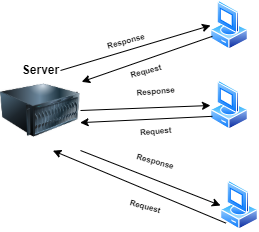
\includegraphics[width=0.50\textwidth]{Backend/client server.drawio.png}
\subsubsection{Welche Arten von Servern gibt es?}

\cite{Server}

\label{server}